\section{Preliminaries}
\label{sec:preliminaries}

\subsection{MPEG decoding}
We first give a brief overview of MPEG decoding and describe how each MPEG video stream shows different CPU usage statistics pattern. 

An MPEG video stream consists of a sequence of still images, that is, frames. 
Each frame is defined as one of three frame types: \term{I-frame} (intrapicture), \term{P-frame} (Predicted picture) or \term{B-frame} (bidirectional predicted picture).
I-frame is self-contained, complete images.  
Thus, no other frames are needed to decode I-frame.
On the other hand, P-frame contains the changes in the image from the previous I-frame or P-frame so it has smaller size than I-frame.
B-frame has an even smaller size than B-frame since it refers a previous and a next I-frame or P-frame, and contains the difference between the previous and the next I-frame or P-frame. 
Overall, I-frames are also most expensive to decode since it involves the computationally expensive \term{Discrete Cosine Transform (DCT)}.
Since each MPEG video stream may have different \term{Group of Pictures (GOP)}, that is, a sequence of frames, GOPs are likely to have different CPU usage patterns. 

When an MPEG video stream is encoded at VBR, different parts in the video stream may require different processing times, mainly due to different data size of P-frame and B-frame. 
The size of P-frame or B-frame is highly variable since they contain only delta information which is the difference from their reference frames i.e. the previous or the surrounding I-frames or P-frames.
In case of a stationary scene, the difference between consecutive frames rarely exists. 
Therefore, the size of P-frame and B-frame can be minimized and, therefore, a less processing time is required to decode the frames.
On the contrary, in case of an action scene where most parts of the image are changing very rapidly, there exists huge difference between consecutive frames.
Therefore, P-frame and B-frame should contain relatively larger data and a more processing time is required to decode.
Since each video stream consists of various types of scenes and a composition of the scenes are also different from each other, CPU usage statistics of each video stream also show different patterns. 

\subsection{Preliminary Experiments}

\begin{figure}[!ht]
	\centering
	\subfigure[Thor] {
		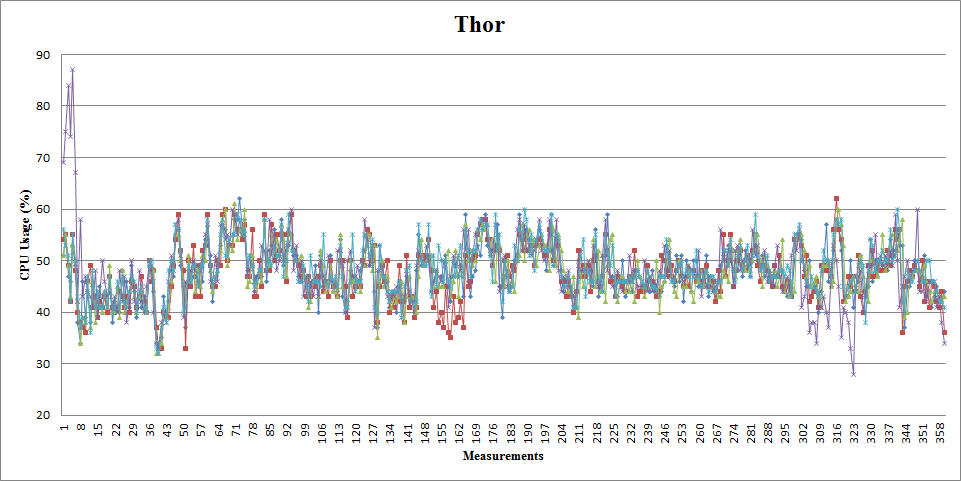
\includegraphics[scale=0.34]{Figures/preliminary_thor}
		\label{fig:preliminary_thor}
	}
	\subfigure[The True Story of Puss 'n Boots] {
		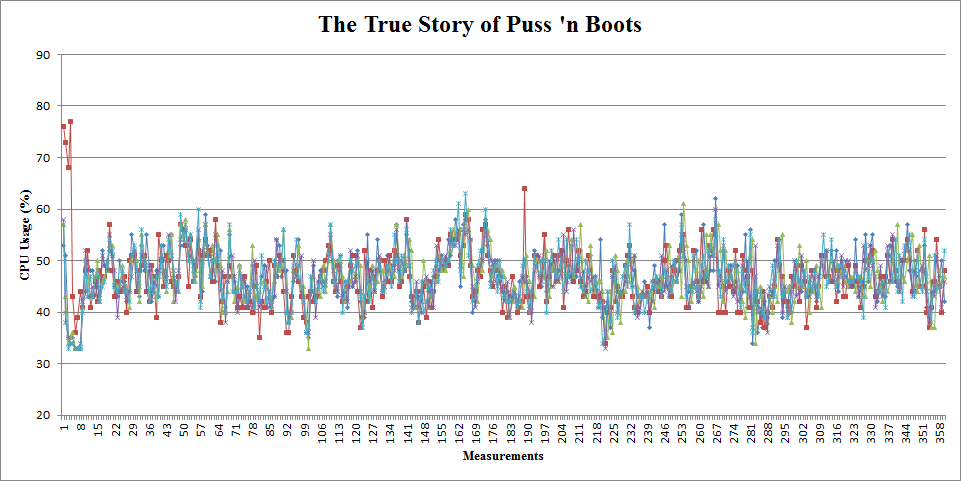
\includegraphics[scale=0.34]{Figures/preliminary_puss}
		\label{fig:preliminary_thor}
	}
	\caption{CPU Usage Measurements of two movies}
	\label{fig:preliminaries}
\end{figure}

In order to make our study feasible, two fundamental conditions should be satisfied: 1) each MPEG video stream shows different and possibly unique CPU usage pattern and 2) repeated measurement on a MPEG video stream show identical CPU usage statistics. 
We show CPU usage statistics collected from two popular movies serviced on Netflix in Figure \ref{fig:preliminaries} and confirm that our assumptions is proved to be correct.
We used Samsung Galaxy S device which was running Android 2.3 Gingerbread and installed Netflix application on the device. 
Measurement interval was set to 5 seconds and we collected CPU usage statistics of first 30 minutes of each movie. 
Per each movie, we repeated the measurement 5 times. 

As shown in Figure \ref{fig:preliminaries}, 5 measurement results on a movie are almost identical in both cases. 
There exist a few exceptional glitches, usually at the initial period during the measurement. 
Our guess is that CPU usage of Netflix application is not deterministic when it starts rendering a movie because of initial buffering.
However, it is later shown by experiments that the existence of glitches would not largely affect our CPU pattern matching algorithm if we apply proper smoothing methods. 

It is also clear from Figure \ref{fig:preliminaries} that two different movies shows clearly different CPU usage statistics. 
If we compare two measurement results using only a few measure points then it may not be easy to differentiate one movie from another.
However if we use enough number of measure points, it would be possible to differentiate each movie from another with reasonably high accuracy. 


